\documentclass{article}
\usepackage{graphicx}
\usepackage[margin=1in]{geometry}
\usepackage[outdir=./]{epstopdf}  					% Avoids errors when input figures
\usepackage[labelsep=period,labelfont=bf]{caption}
%\usepackage{subcaption}

\begin{document}

\begin{figure}[tbph]
	\caption{Monetary Policy Surprises in Mexico} \label{fig:factorslines}
	\begin{center}									% center the minipage on the line
		\begin{minipage}{0.9\linewidth}
			\begin{center}							% center the figure inside the minipage
				\includegraphics[trim={0cm 0cm 0cm 0cm},clip,height=.4\textheight,width=\linewidth,keepaspectratio]{filename} \\
			\end{center}
			\fignotes{Details.}
		\end{minipage}
	\end{center}
\end{figure}

% trim = {<left> <lower> <right> <upper>}
%	\vspace{-0.4cm} \caption*{\footnotesize{\textit{Notes}: Notes.}}

%\begin{figure}[tbph]
%	\caption{Connectedness of the Term Structure} \label{fig:dy_index_ts}
%	\begin{center}
%		\begin{minipage}{0.9\linewidth}
%			\begin{center}
%				\begin{subfigure}[t]{\linewidth}
%					\includegraphics[trim={0cm 0cm 0cm 0cm},clip,height=0.38\textheight,width=\linewidth]{../Figures/Estimation/dy_index_ts.eps} \\
%					\vspace{-0.35cm}
%					\caption{Emerging Markets} \label{subfig:dyindexTSEM}
%					\vspace{0.4cm}
%				\end{subfigure}
%				
%				\begin{subfigure}[t]{\linewidth}
%					\includegraphics[trim={0cm 0cm 0cm 0cm},clip,height=0.38\textheight,width=\linewidth]{../Figures/Estimation/dy_index_ts_AE.eps} \\
%					\vspace{-0.35cm}
%					\caption{Advanced Countries} \label{subfig:dyindexTSAE}
%				\end{subfigure}
%			\end{center}
%			\fignotes{Details.}
%		\end{minipage}
%	\end{center}
%\end{figure}

\end{document}

% Put image and its description into a minipage environment
%https://tex.stackexchange.com/questions/102516/note-below-figure-as-long-as-the-figure-all-centered-but-note-left-aligned

% minipage description
%http://joshua.smcvt.edu/latex2e/minipage.html

%Align caption to the left
%https://tex.stackexchange.com/questions/275131/align-caption-to-the-left